Freefall problems frequently occur in elementary physics examinations. These types questions normally follow a pretty standard format, as follows. First, a projectile has been launched from a certain angle at a certain velocity. Second, you will be asked to find something such as the total distance traveled by the projectile. The good thing about these problems is that once you understand them, they are simple. The difficult part of these problems is recognizing how the gravitational force only impacts a force in the vertical direction and that therefore the horizontal velocity of the projectile will remain constant throughout the flight of the projectile. I will not discuss them here as I find them to be more fun to solve on your own using the facts that I have been given. However, one other fact may prove useful. That is, at the peak of the flight of a projectile, the vertical velocity of the projectile must be 0. I urge you to think about this point for a little bit, and it should start to make sense. 
\newline
\newline
\newline
\newline
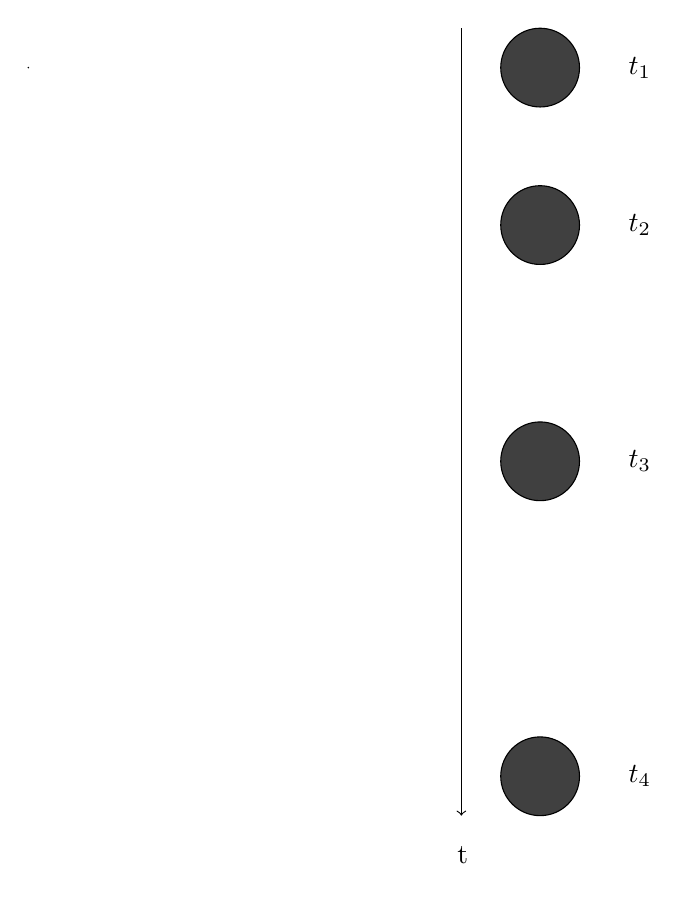
\begin{tikzpicture}
\filldraw[fill = darkgray, draw = black] (0,0) circle (0.001cm);
\filldraw[fill = darkgray, draw = black] (6.5,0) circle (0.5cm);
\filldraw[fill = darkgray, draw = black] (6.5,-2) circle (0.5cm);
\filldraw[fill = darkgray, draw = black] (6.5,-5) circle (0.5cm);
\filldraw[fill = darkgray, draw = black] (6.5,-9) circle (0.5cm);
\draw[->] (5.5,0.5) -- (5.5,-9.5);
\draw[black] (5.325,-10) node[anchor=west] {t};
\draw[black] (7.5,0) node[anchor=west] {$t_1$};
\draw[black] (7.5,-2) node[anchor=west] {$t_2$};
\draw[black] (7.5,-5) node[anchor=west] {$t_3$};
\draw[black] (7.5,-9) node[anchor=west] {$t_4$};
\end{tikzpicture}
\newline
\newline
\newline
\newline